\documentclass{article}
\usepackage[utf8]{inputenc}
\usepackage{graphicx}

\title{Misura della costante di Planck mediante Corpo Nero}
\author{Francesco Pio Merafina, Onofrio Davide Caputo, Alessandro Lamesta}
\date{}
\begin{document}
\maketitle
\section{Abstract:}
Si vuole misurare la costante di Planck studiando l’emissione di radiazione elettromagnetica da parte di un filamento di tungsteno portato all’incandescenza
~
\section{Cenni teorici:}
La teoria alla base dell'esperimento è quella di sfruttare una lampadina ed osservarne lo spettro in funzione della temperatura, per poi ricavare la costante di Planck.
~
\section{Apparato sperimentale:}
L'apparato consiste in una lampadina a filamento di Tungsteno, uno spessimetro, un calibro, un tester digitale, un fotodiodo, un filtro ottico che fa passare solo luce con lunghezza d'onda 520nm con banda passante 40nm, una resistenza da 1.7M$\Omega$, un voltmetro in parallelo alla lampadina ed un amperometro in serie alla lampadina, ed un generatore di tensione che alimenta la lampadina, un proiettore e carta millimetrata.
~
\section{Metodologia di misura:}
Per eseguire l'esperimento abbiamo prima di tutto misurato le dimensioni lineari della spira per poterne calcolare la superficie:
\begin{itemize}
    \item n = numero spire = 19
    \item s = diametro spire = 0.250mm ± 0.025mm
    \item l$_{1}$ = lato 1 filaemento = 4.5mm ± 0.2mm
    \item l$_{2}$= lato 2 filamento = 1.0mm ± 0.2mm
\end{itemize}
Dopo aver trovato queste misure, si passa a riscaldare il filamento di Tungsteno, il quale emette ad una temperatura T che dipende dalla potenza dissipata che si ottiene come prodotto della tensione ai capi del filamento per la corrente che scorre in esso; e per fare ciò si utilizzano un voltmetro in parallelo ed un amperometro in serie. Per misurare la corrente che scorre a causa dell fotodiodo, essendo molto bassa si usa una resistenza molto grande che in parallelo ha un tester Per la misura dell'emissività del tungsteno si procede in maniera iterattiva sfruttando dei valori tabulati, ponendo prima $\epsilon$ = emissività = 1, si calcola la temperatura, si ottiene l'emissività a partire dalla tabella, si ricalcola la temperatura, e si procede in maniera iterativa fino alla convergenza. Per gli errori si deve prima di tutto considerare gli errori sulla misura delle due tensioni, sul filamento, il quale è molto sensibile, ed anche della corrente che scorre.
~
\section{Analisi dati:}
Prima di procedere alla effettiva analisi dati si sono valutate le incertezze, la prima ad essere stata valutata è quella della superficie, la quale si ottiene come:
\begin{equation}
    A=n\pi s(2l_{1}+2l_{2})=(168\pm 19)mm^{2}
\end{equation}
Quindi propagando l'errore otteniamo l'incertezza. Dopo questa prima incertezza importante, vanno considerata l'incertezza sulla banda passante dal filtro, il quale fa passare una lunghezza d'onda di 520nm±20nm. Ora di seguito verrano riportate le formule usate per l'analisi dei dati:
Legge di Joule:
\begin{equation}
    P=VI
\end{equation}
Intensità della radiazione e.m. che investe l'apparato sperimentale, di un corpo con emissività $\epsilon$, alla temperatura T:
\begin{equation}
    J(T)=fR(\nu,T)\Delta\nu
\end{equation}
f è la frazione di potenza emessa dal filamento che arriva sul fotodiodo, R la radianza spettrale, $\Delta\nu$ è l'intervallo di frequenze che passano il filtro ottico.
Radianza spettrale, Legge di Planck:
\begin{equation}
    R(\nu,T)=\epsilon\frac{8\pi h\nu^3}{c^2e^\frac{h\nu}{kt}-1} \sim \epsilon\frac{8\pi h\nu^3}{c^2}e^\frac{-h\nu}{kt}
\end{equation}
L'approssimzione si è fatta poiché h$\nu>>$  kT, infatti h$\nu\sim$ 2.2/2.5 eV, mentre kT è $\sim$0.1eV.
Legge di Stefan:
\begin{equation}
    P=\epsilon\sigma AT^4
\end{equation}
La costante di Stefan vale:
\begin{equation}
    \sigma=\frac{2\pi^5k^4}{15h^3c^2}
\end{equation}
Per trovare il valore di h si esegue il rapporto tra due diversi valori di J, $\epsilon$, P:
\begin{equation}
    h=b*\frac{P_{1}P_{2}}{(\epsilon_2P_1)^\frac{1}{4}-(\epsilon_1P_2)^\frac{1}{4}}(ln\frac{J_1}{J_2}-ln\frac{\epsilon_1}{\epsilon_2})^4
\end{equation}
\begin{equation}
    b=\frac{15c^2}{2\pi^5 A\nu^4}
\end{equation}
~
\section{Risultati e conclusioni:}
Osservando i grafici di figura 1,2 si può osservare come il valore della costante di Planck misurato sia h=(6.61$\pm$0.06)10$^{-34}$Js
compatibile con il valore vero di h=6.63*10$^{-34}$Js
~
\section{Grafici e Tabelle:}
\begin{figure}[h!]
    \centering
    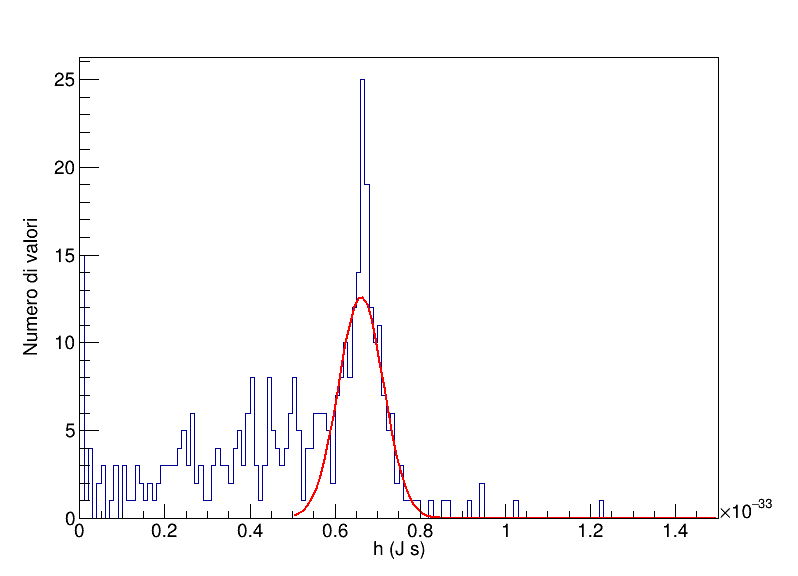
\includegraphics[width=\linewidth]{h_dist.png}
    \caption{Distribuizione gaussiana dei valori della costante di Planck ottenuti usando la formula 6}
    \label{figura1}
\end{figure}
\begin{figure}[h!]
    \centering
    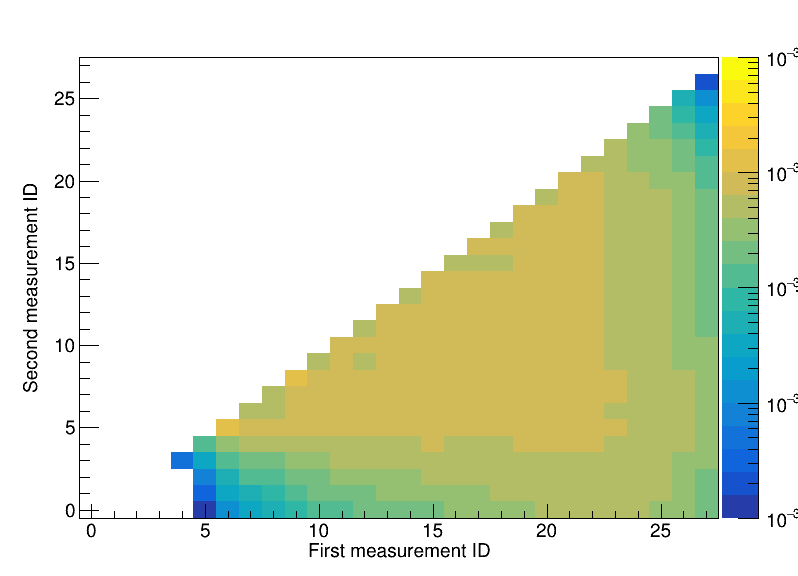
\includegraphics[width=\linewidth]{h_values.png}
    \caption{Diagramma rappresentante il valore della costante di Planck, ottenuto dalla particolare coppia di dati relativa al primo e al secondo set di misure, in correlazione al gradiente cromatico.}
    \label{figura1}
\end{figure}
\begin{figure}[h!]
    \centering
    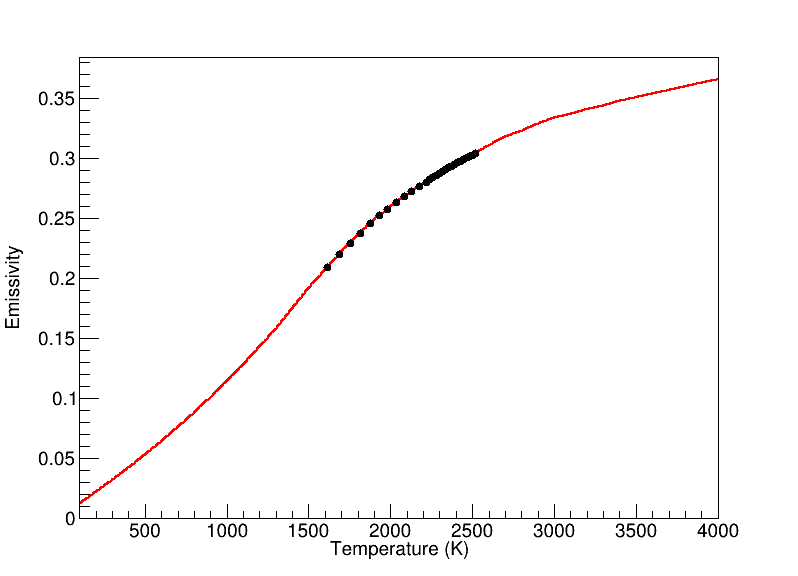
\includegraphics[width=\linewidth]{emissivity.png}
    \caption{Andamento dell'emissività in funzione della temperatura}
    \label{figura1}
\end{figure}
\begin{table}[h!]
  \begin{center}
   \begin{tabular}{|c|c|c|c|}
      V$_{L}$[V]&I$_{L}$[A]&V$_{PD}$[V]&V$_{FD}$[V]\\
      17.73&6.58&4.53&20\\
      17.35&6.50&4.53&20\\
      17.00&6.42&4.49&20\\
      16.75&6.37&4.49&20\\
      16.30&6.28&4.33&20\\
      15.95&6.20&4.08&20\\
      15.60&6.13&3.70&20\\
      15.25&6.05&3.38&20\\
      14.90&5.97&3.07&20\\
      14.55&5.90&2.78&20\\
      14.20&5.82&2.52&20\\
      13.85&5.74&2.25&20\\
      13.50&5.66&2.04&20\\
      13.15&5.58&1.81&20\\
      12.80&5.50&1.62&20\\
      12.45&5.42&1.43&20\\
      12.10&5.33&1.27&20\\
      11.40&5.16&0.98&20\\
      10.70&4.98&0.74&20\\
      10.00&4.80&0.54&20\\
      9.30&4.62&0.39&20\\
      8.60&4.42&0.26&20\\
      7.90&4.23&0.18&20\\
      7.20&4.02&0.12&20\\
      6.50&3.80&0.078&2\\
      5.80&3.58&0.051&2\\
      5.10&3.35&0.036&2\\
      4.40&3.10&0.029&2\\
   \end{tabular}
  \caption{Tabella associata al primo grafico}
  \end{center}
\end{table}
 











\end{document}